% 2018 May 22 - From Jackson+ (2013) study of HAT-P-7 - "Welsh et al. (2010) discovered ellipsoidal variations in the Kepler Q1 data, with an amplitude of 37.3 ppm. They also estimated that the planet’s phase curve has an amplitude of 31.9 ppm..." - So EVs and planet's phase curve has comparable amplitudes.

\documentclass[manuscript]{aastex}

%% preprint2 produces a double-column, single-spaced document:

%% \documentclass[preprint2]{aastex}

%% Sometimes a paper's abstract is too long to fit on the
%% title page in preprint2 mode. When that is the case,
%% use the longabstract style option.

%% \documentclass[preprint2,longabstract]{aastex}

%% If you want to create your own macros, you can do so
%% using \newcommand. Your macros should appear before
%% the \begin{document} command.
%%
%% If you are submitting to a journal that translates manuscripts
%% into SGML, you need to follow certain guidelines when preparing
%% your macros. See the AASTeX v5.x Author Guide
%% for information.

\newcommand{\kepler}{{\it Kepler}}
\newcommand{\tess}{{\it TESS}}
% \newcommand{\myemail}{skywalker@galaxy.far.far.away}

%% You can insert a short comment on the title page using the command below.

\slugcomment{Submitted to ApJ, Fall 2018}

%% If you wish, you may supply running head information, although
%% this information may be modified by the editorial offices.
%% The left head contains a list of authors,
%% usually a maximum of three (otherwise use et al.).  The right
%% head is a modified title of up to roughly 44 characters.
%% Running heads will not print in the manuscript style.

\shorttitle{Eclipse Variability}
\shortauthors{Jackson, Sandidge, Kreyche, \& Briggs}

%% This is the end of the preamble.  Indicate the beginning of the
%% paper itself with \begin{document}.
\usepackage{hyperref}
\usepackage{graphics,graphicx}

\begin{document}

%% LaTeX will automatically break titles if they run longer than
%% one line. However, you may use \\ to force a line break if
%% you desire.

\title{Searching for Variability in Eclipses in the Kepler Dataset}

%% Use \author, \affil, and the \and command to format
%% author and affiliation information.
%% Note that \email has replaced the old \authoremail command
%% from AASTeX v4.0. You can use \email to mark an email address
%% anywhere in the paper, not just in the front matter.
%% As in the title, use \\ to force line breaks.

\author{Brian Jackson\altaffilmark{1}, Wesley Sandidge, Steven Kreyche, \& Jennifer Briggs}
\affil{Department of Physics, Boise State University\\ 1910 University Drive, Boise ID 83725-1570 USA}

%% Notice that each of these authors has alternate affiliations, which
%% are identified by the \altaffilmark after each name.  Specify alternate
%% affiliation information with \altaffiltext, with one command per each
%% affiliation.

\altaffiltext{1}{bjackson@boisestate.edu}

%% Mark off your abstract in the ``abstract'' environment. In the manuscript
%% style, abstract will output a Received/Accepted line after the
%% title and affiliation information. No date will appear since the author
%% does not have this information. The dates will be filled in by the
%% editorial office after submission.

\begin{abstract}

Exoplanetary eclipses occur when a planet passes behind its host star, causing the planet’s reflected and emitted light to be blocked. We search for variability in the eclipses of the short period hot Jupiter HAT-P-7b using data from NASA’s Kepler mission. This variability could provide insight into the meteorology of the planet and how the atmosphere changes with each orbit. The model phase curve is composed of three signals: the planetary reflected and emitted radiation, ellipsoidal variations due to tidal forces acting on the planet, and Doppler flux variations due to reflex motion with the host star as well as instrumental effects. The relationship between these signals, as well as the transit, may allow for planetary variability to be distinguished from other forms of variability. We will apply this model to all of the available data and perform fits to the transit and eclipse of each orbit. The optimal number of eclipses will be stacked to improve the signal-to-noise ratio while preserving any detectable variability.

\end{abstract}

%% Keywords should appear after the \end{abstract} command. The uncommented
%% example has been keyed in ApJ style. See the instructions to authors
%% for the journal to which you are submitting your paper to determine
%% what keyword punctuation is appropriate.

\keywords{globular clusters: general --- globular clusters: individual(NGC 6397,
NGC 6624, NGC 7078, Terzan 8}

%% From the front matter, we move on to the body of the paper.
%% In the first two sections, notice the use of the natbib \citep
%% and \citet commands to identify citations.  The citations are
%% tied to the reference list via symbolic KEYs. The KEY corresponds
%% to the KEY in the \bibitem in the reference list below. We have
%% chosen the first three characters of the first author's name plus
%% the last two numeral of the year of publication as our KEY for
%% each reference.


%% Authors who wish to have the most important objects in their paper
%% linked in the electronic edition to a data center may do so by tagging
%% their objects with \objectname{} or \object{}.  Each macro takes the
%% object name as its required argument. The optional, square-bracket 
%% argument should be used in cases where the data center identification
%% differs from what is to be printed in the paper.  The text appearing 
%% in curly braces is what will appear in print in the published paper. 
%% If the object name is recognized by the data centers, it will be linked
%% in the electronic edition to the object data available at the data centers  
%%
%% Note that for sources with brackets in their names, e.g. [WEG2004] 14h-090,
%% the brackets must be escaped with backslashes when used in the first
%% square-bracket argument, for instance, \object[\[WEG2004\] 14h-090]{90}).
%%  Otherwise, LaTeX will issue an error. 


\section{Introduction}


\section{Modeling the HAT-P-7 System}

stellar parameters for HAT-P-7 taken from \citet{2012ApJ...757..161T}.

Here is an equation: $\vec{F} = m \vec{a}$.
\begin{equation}
\vec{F} = m \vec{a}
\end{equation}

\subsection{Model Phase Curve}

	The model phase curve of HAT-P-7b is composed of three signals: the planetary reflected and emitted radiation, ellipsoidal variations due to tidal forces acting on the planet, and Doppler flux variations due to reflex motion with the host star as well as instrumental effects. These signals are additive to form a resultant phase curve that models the relative flux contribution of the planet compared to its star. The baseline flux is defined to be 0 as the stellar flux that would be received from the host star in the absence of a planet. In order maintain consistency with this set baseline, the modeled planetary and ellipsoidal signals were shifted so that their minimums lie at the baseline. The Doppler variations signal was left to range from positive and negative contributions, with the signal centered at the baseline. It is important to note that the functions constructed to output these signals were written in terms of the amplitudes of their signals rather than the entire signal.

\subsection{Model Eclipse}

    To complete the necessary functions needed to model the entire orbit of HAT-P-7b, the transit and eclipse were incorporated. This was accomplished with the use a Python code written by Jason Eastman called occultquad. The occultquad code outputs the transit and occultation curves after taking the arguments of the projected varying distance between the planet and star, the quadratic limb darkening coefficients, and the ratio of the planet to stellar radii. 
    The eclipse was generated by approximating the limb darkening coefficients to be equal to 1, while using the square root of the eclipse depth rather than the radii ratio. This output was then shifted by its minimum and divided through by its maximum to ensure that the signal ranged from 0 to 1. This output was multiplied by the planetary phase curve signal to construct the model eclipse with the bottom at the defined baseline.
    
\subsection{Model Transit}

    The transit was generated by using the limb darkening coefficients as found by Claret and Bloemen (2011), along with the ratio of radii parameter as found in Welsh et. al (2010). The output transit signal was subtracted by 1 in order to ensure that its maximum was at the defined baseline. The signal was outputted with the use of super sampling in order to improve the accuracy of the model. 
    The eclipse and transit were both incorporated into one function along with the model phase curve that allows for the output of the continuous lightcurve of an orbit. This will allow both the eclipse and transit to be fit simultaneously with the Kepler data which will allow for thorough analysis of variability. 


Citation needed for Jason Eastman occultquad code

Citation needed for Claret and Bloemen (2011)

Citation needed for  Welsh et. al (2010)


\section{Data Analysis}
For each system's light curve, we applied the following steps to condition each quarter's data:
\begin{enumerate}
\item We subtracted the median value from each quarter's PDCSAP\_FLUX time-series, before dividing through by the median.
\item We next applied a median boxcar filter with a window size equal to an integer number of orbital periods for the target -- for each system, we considered $n$ from one up to five, choosing the value that maximizes the eclipse signal when we fold together all the available data on the best-fit orbital period from previous analyses. To mitigate edge-effect distortions, we extended the time-series beyond both ends out a full window length by reflecting the original time-series across its boundary.
\item Finally, we stitched each quarter's conditioned data into one long time-series and subtracted the average value of the planet's eclipse (i.e., we zeroed out the eclipse) because, in principle, only the star's light registers during that phase so it sets the baseline against which to measure the photometric variations.
\end{enumerate}
Figure \ref{fig:Analysis_of_Kepler76b_data} illustrates a portion of the raw and conditioned time-series for Kepler-76 b. After pursuing the above data conditioning procedure, we using the Levenburg-Marquardt to fit a standard transit light curve \citep{2002ApJ...580L.171M} to the mid-transit times for all the transits in each dataset and confirmed they conformed to a linear ephemeris, finding no evidence for transit-timing variations. Below we report new ephemerides slightly updated relative to previous analyses for each object.

\begin{figure}
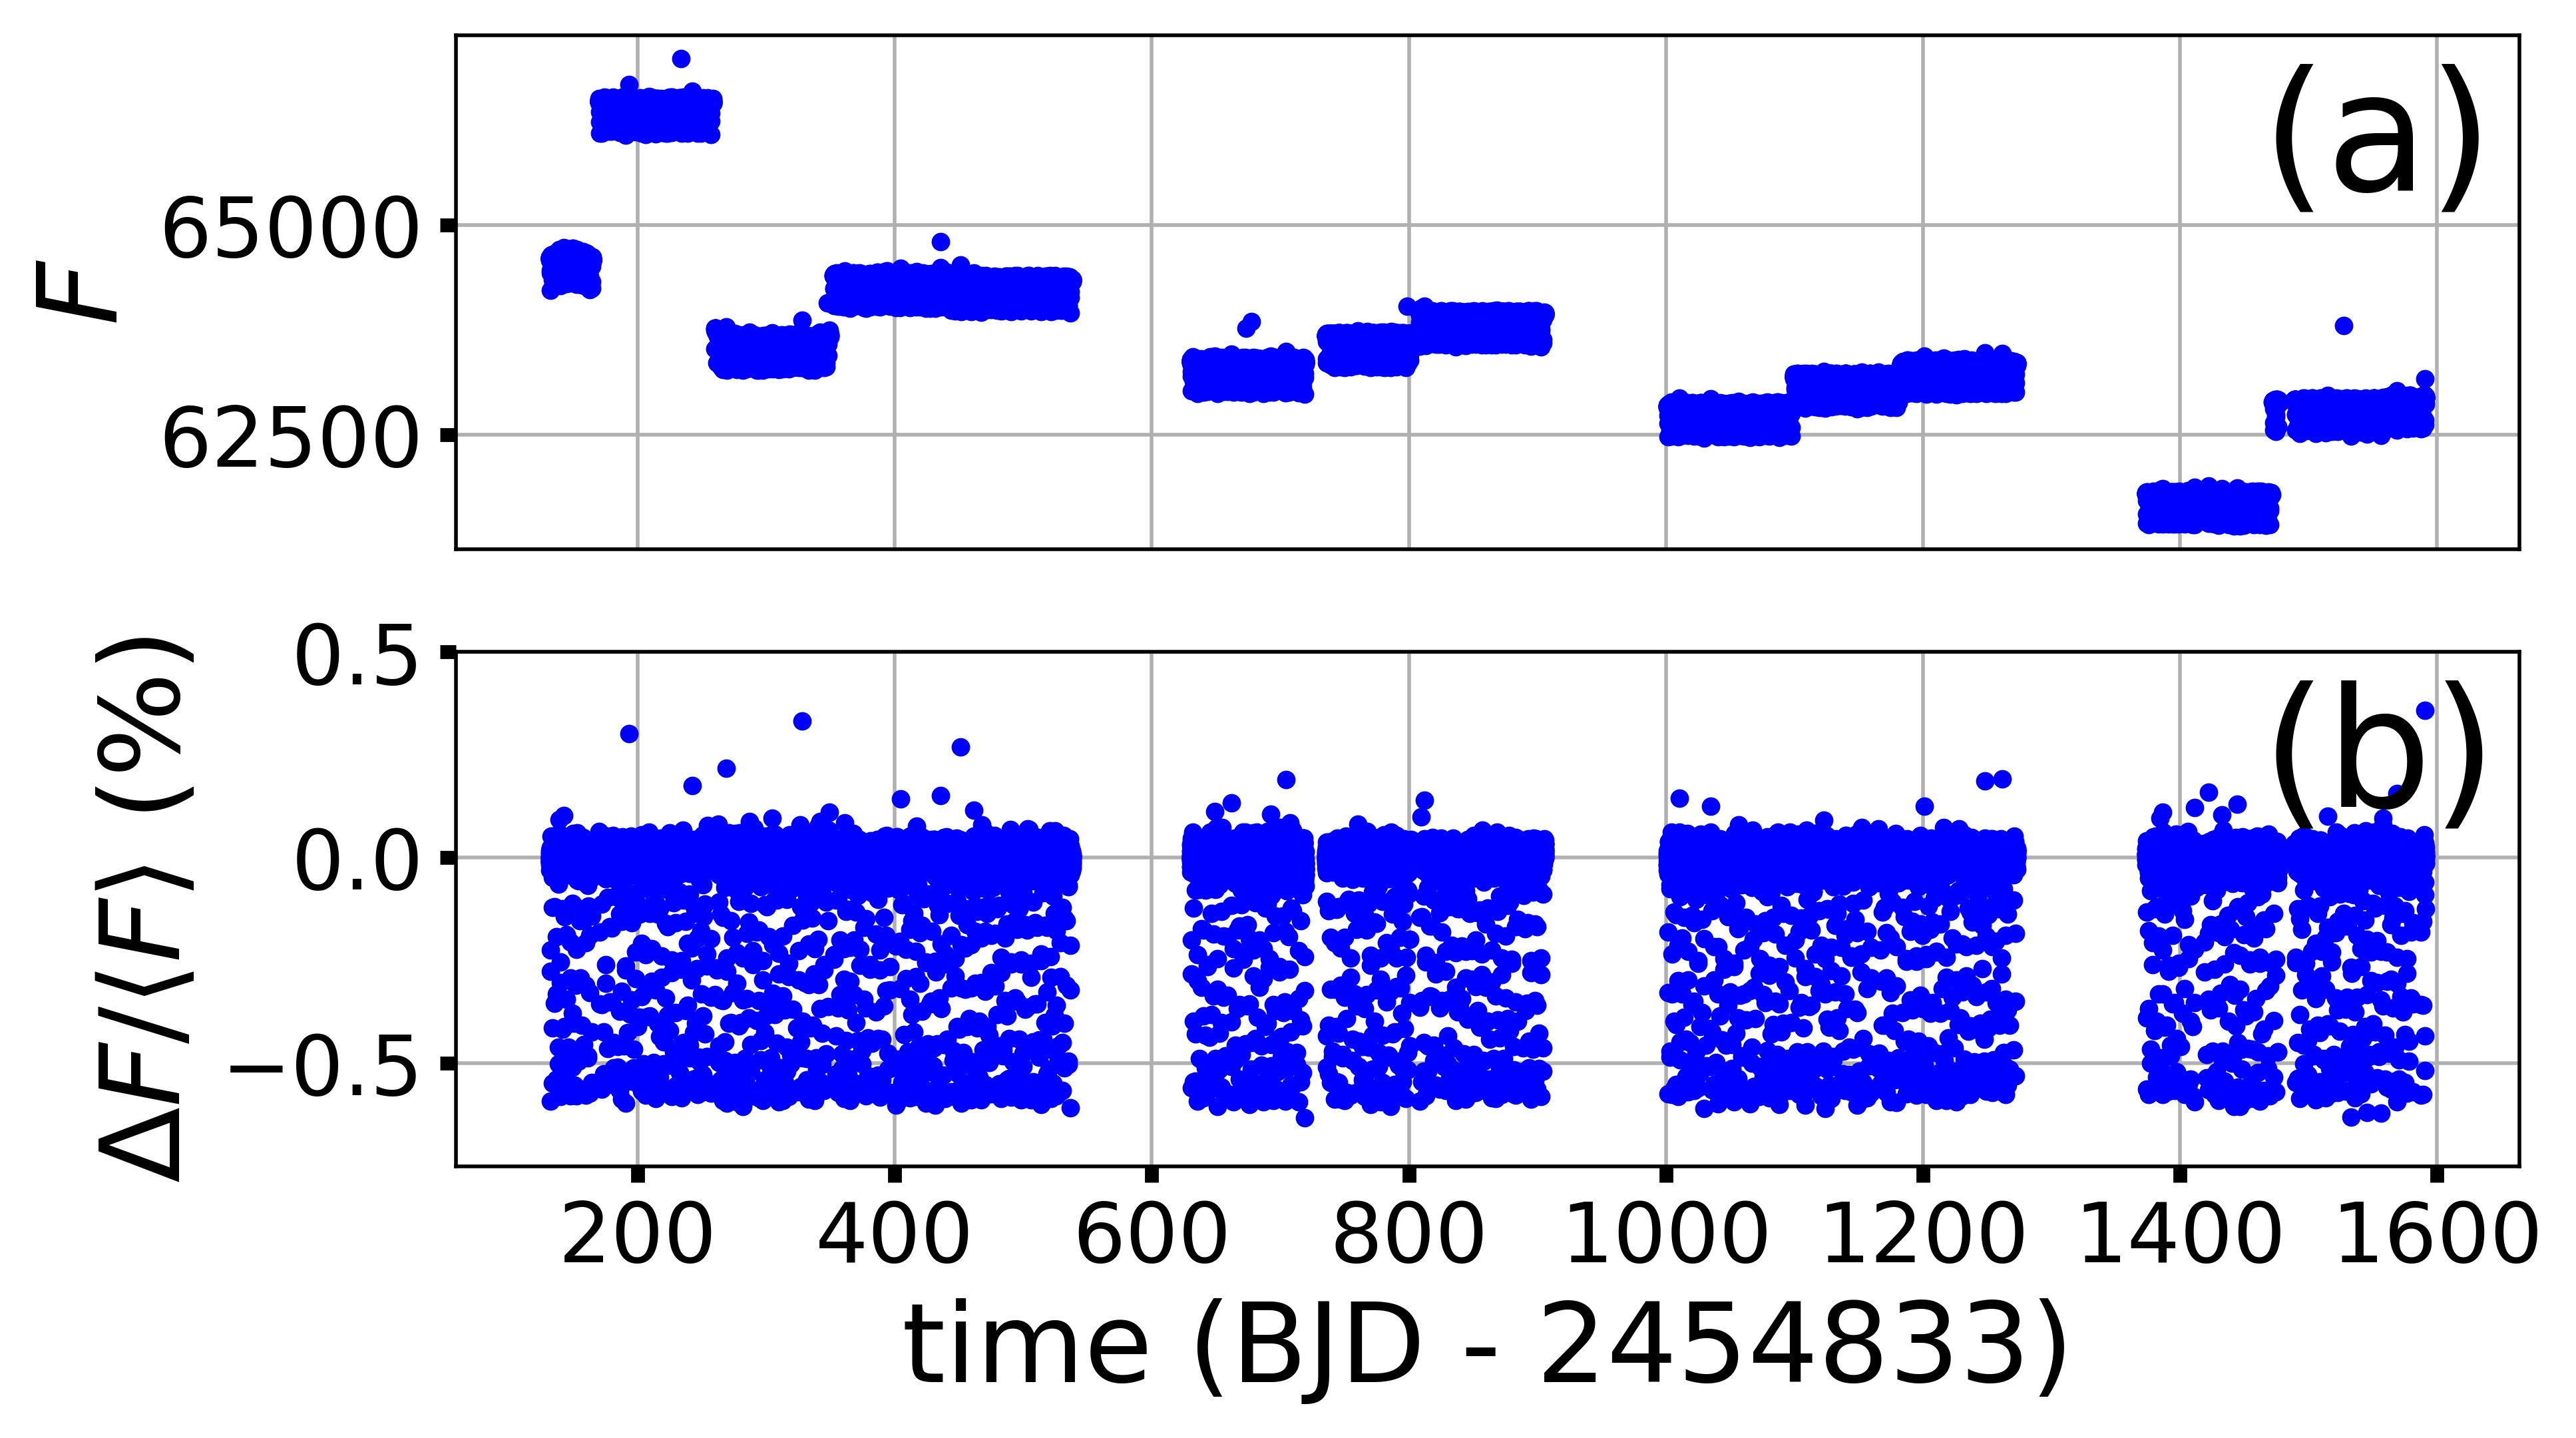
\includegraphics[width=0.5\textwidth]{Analysis_of_Kepler76b_data.jpg}
\caption{The quarter-by-quarter Raw (a) and conditioned (b - in \%) PDCSAP\_FLUX. Time along the x-axis is shown in the \kepler\ mission's barycentric Julian date minus 2454833 (midnight on 2009 January 1), and the y-axis shows variations in flux. \label{fig:Analysis_of_Kepler76b_data}}
\end{figure}



\section{Examination of Variability}

\subsection{Signals and Their Relationships}

	The search for variability in the eclipse of HAT-P-7b will require a careful analysis of the signals that compose its lightcurve. Planetary variability must be able to be distinguished from other forms of variability in order to gain useful insight into the system. This can be accomplished by examining the relationship between the planetary reflected and emitted radiation signal as the eclipse depth with the other signals that comprise the phase curve along with the transit signal. With the model functions constructed to produce and fit these signals, the correlation relationships between these signals can be examined while variability is present. 
    
	These correlation relationships can be tested through controlled synthetic data that mimics the nature of the real data from Kepler. This was done by first obtaining the standard deviation of the noise present in the Quarter-2 unbinned lightcurve data, which was folded over one orbital period with the transit masked. The standard deviation was obtained from the residuals after subtracting the data by the model curve inputted with the standard parameters from Jackson (2012). This standard deviation was used to inject into the synthetic data using a random Gaussian distribution.
    
    For each pair of signals examined, a random uniform distribution was used to produce a random value for each parameter within ten percent of the standard value as found in Jackson (2012). Many iterations were run to randomly fluctuate these parameters, generating a synthetic lightcurve each time with the new values. The lightcurves were then fit to attempt to re-obtain these values each iteration, gathering the uncertainties of these fit results. Plotting the uncertainties of the fits of both parameters against each other for each case allows for the correlation to be examined in a useful visual. 

Citation needed for Jackson (2012)

\subsection{Planetary Eclipse and Transit Variability} 

	One key case to examine with the search for variability in the eclipse is to explore how it relates to variability in the transit. Consider that the depth of the eclipse is found to be variable from orbit to orbit through analysis of data fitting. This information alone does not allow for any firm conclusions to be made about the source of the variability. This variability could just as well be a result of an planetary change such as cloud coverage moving in, as a form of stellar variability such as a star spot. It is important to consider that this stellar variability must have a duration that exists roughly longer than the orbital period of the planet.

	Figure 1 shows a diagram depicting an event of stellar variability, in which a transiting planet crosses the disk of its host star as a star spot is present on the surface. Assuming we neglect the contribution of flux from the region of the star covered by the star spot, the total surface area of the star's disk has been reduced. This means that we expect the observed transit to be deeper due to the transit depth being directly dependent on the ratio of the planet and star's disc surface areas. The plot included to the right of this diagram shows the relative flux plotted against the phase position as the planet transits the star. The solid red transit curve shows the transit depth in the absence of the star spot, while the dotted blue line shows the expected deepening in the transit due to the star spot.
    
    Figure 2 follows this idea by depicting the other half planet's orbit, showing what is expected in the event of stellar variability while the planet is eclipsed. The diagram shows that on behalf of the star, nothing has changed and the star spot is still acts to reduce the stellar disk's total flux-contributing surface area. The planet is shown as a green outline behind the star, where a dip in flux occurs due to the loss of flux from the planetary source. Like the transit, the eclipse depth is also expected to deepen, where the relative flux lost between the planet and star is again dependent on their available surface areas. A similar plot is again shown to the right of this diagram, where the solid red line represents the eclipse curve without any stellar variability present. The dotted blue line shows what an observation of the eclipse curve would be with the star spot present, a deeper eclipse. 
    
    Gathering from this understanding, the transit and eclipse signals are affected identically in the presence of stellar variability, where they will change by the same relative amount. The transit and eclipse will be simultaneously be fit during the analysis to check whether any detected variability is deemed to be stellar variability or planetary variability in the eclipse. To clarify, if both curves are found to  vary in an orbit, then it suggests stellar variability. However, if the eclipse depth is found to vary but the transit depth does not, then the source of the variability was likely due to planetary changes.
 
	The correlation relationship must be known between the transit and eclipse depth signals in order to enact the previously described process. These signals must be independent of one another and show no correlation. This means that carrying out the discussed process of injecting random variability into the synthetic data should yield a plot of fit uncertainties with the appearance of random scatter. Looking to figure 3, this test was carried out, showing the uncertainty in the eclipse depth plotted on the vertical axis against the uncertainty in the transit depth on the horizontal axis. The plot is promising, and does not appear to reveal any notable correlation between these signal parameters, where the distribution is evenly spread out in a random nature. This concludes that the transit signal can be used with the planetary eclipse signal as a check while searching for variability. Figure 4 shows a single fit result of the many iterations carried out, where the same plot is shown on different scales to show both the transit and eclipse.


\subsection{Planetary Eclipse and Ellipsoidal Variability} 

	It will also be useful to know the relationship between the eclipse signal and the ellipsoidal variation signal that is also present in the phase curve of HAT-P-7b. Figure 5 shows a similar plot from before, where this time the uncertainty in the eclipse depth is plotted on the vertical axis against the uncertainty in the ellipsoidal variation signal on the horizontal axis. This time, the results show that there appears to be a distinguishable trend in the plotted fit uncertainties. The uncertainties and therefore the signals appear to be linearly correlated in the presence of variability. This means that these two signals could not be used as checks in the same manner as the uncorrelated transit and eclipse signal. Figure 6 again shows a single fit result of the lightcurve.
   

\subsection{Planetary Eclipse and Ellipsoidal Variability} 

Lastly, it could also prove worthwhile to examine the relationship between the eclipse signal and the Doppler flux variation signal when influenced by variability. Performing the test, the plotted uncertainties as seen in figure 7 show the uncertainty of the eclipse depth on the vertical axis versus the uncertainty in the Doppler flux variation signal on the horizontal axis. The results show as random scatter that there does not appear to be any correlation between these two signals. There is a possibility that this result comes from the amplitude of the Doppler flux variation signal being much smaller than the planetary eclipse signal, where the fits were not precise enough to detect anything of significance. 


\section{Data Conditioning}

	This project aims to use and analyze all of the available data for HAT-P-7b from the Kepler dataset. The quarter-2 raw light curve data was first obtained for the testing of initial project goals. This raw data was conditioned to eliminate as much noise and troublesome outliers as possible. To accomplish this, a high-pass filter called a boxcar filter was applied to ensure that any repetitive high frequency signals were kept. The rare, low frequency signals were discarded as outliers. All invalid values present as errors in the dataset within the time and corrected flux arrays were removed. The arrays were linearly interpolated, and the sampling frequency calculated from the time array was used to apply a median filter to the data, removing outliers that exceeded 10 sigma. 
    
    The signal of the eclipse is largely imperceptible when looking at a single orbit. The quarter-2 data file consists of about 40 orbits, which were folded over the planet's orbital period. The stacked eclipses reveal a perceptible signal. The data was finally converted from time space ranging from the start to end of the orbit, to the orbital phase position of the planet. This was done using the center of transit value in BJD taken from Pal et. al (2008) to shift the data in accordance with Kepler's baseline time. The eclipse was set to be centered at the phase position of 0.5, where the phase position is defined to span from 0 to 1. 

\subsection{Model Fitting}

%% In this section, we use  the \subsection command to set off
%% a subsection.  \footnote is used to insert a footnote to the text.

%% Observe the use of the LaTeX \label
%% command after the \subsection to give a symbolic KEY to the
%% subsection for cross-referencing in a \ref command.
%% You can use LaTeX's \ref and \label commands to keep track of
%% cross-references to sections, equations, tables, and figures.
%% That way, if you change the order of any elements, LaTeX will
%% automatically renumber them.

%% This section also includes several of the displayed math environments
%% mentioned in the Author Guide.

\section{Results}

%% The \notetoeditor{TEXT} command allows the author to communicate
%% information to the copy editor.  This information will appear as a
%% footnote on the printed copy for the manuscript style file.  Nothing will
%% appear on the printed copy if the preprint or
%% preprint2 style files are used.

%% The eqnarray environment produces multi-line display math. The end of
%% each line is marked with a \\. Lines will be numbered unless the \\
%% is preceded by a \nonumber command.
%% Alignment points are marked by ampersands (&). There should be two
%% ampersands (&) per line.


%% If you wish to include an acknowledgments section in your paper,
%% separate it off from the body of the text using the \acknowledgments
%% command.

%% Included in this acknowledgments section are examples of the
%% AASTeX hypertext markup commands. Use \url without the optional [HREF]
%% argument when you want to print the url directly in the text. Otherwise,
%% use either \url or \anchor, with the HREF as the first argument and the
%% text to be printed in the second.

\section{Discussion and Conclusions}
Figure \ref{fig:eclipse_estimates} shows estimates of signal-to-noise ratios (SNR) expected for secondary eclipses observed by \tess\ based on the synthetic population of planets in the \tess\ yield calculations from \citet{2018arXiv180405050B}. For each synthetic planet from that study, we estimated the eclipse depth $\Delta$ for the case that the planet reflects all of the light it receives from the star (shown in blue) and for the case that the planet emits (and absorbs) light as a perfect blackbody (shown in orange). For the former case, the eclipse depth is given as $\frac{1}{4} \left( \frac{R_{\rm p}}{a} \right)^2$, where $R_{\rm p}$ is the planetary radius and $a$ is the orbital semi-major axis. We then estimated the corresponding SNR by multiplying the transit SNRs given for each planet by planet-star radius ratio squared and then by $\Delta_{\rm reflected}$. For the latter case, we used the stellar insolation given for each planet and assumed dayside thermal equilibrium with zero albedo for each planet to estimate a brightness temperature and convolved the resulting blackbody curve against the \tess\ spectral response function\footnote{https://tessgi.github.io/TessGiWebsite/the-tess-space-telescope.html}. We combined the insolation and planet's orbital distance to estimate the stellar effective temperature and, likewise, convolved the corresponding blackbody curve against the response function. Finally, we divided the planet's convolved brightness by the star's and used the re-scaled transit SNR to calculate the SNR for the thermally emitted eclipse. Figure \ref{fig:eclipse_estimates} only shows those SNR-values $> 3$, among which the vast majority (54 of 62 total) have $R_{\rm p} \geq 10\ R_{\rm Earth}$.

The synthetic population from \citet{2018arXiv180405050B} included 4,553 planets, and Figure \ref{fig:eclipse_estimates} suggests only about 1\% of these may have secondary eclipses detectable for \tess\. However, among those, our calculation suggests that the eclipse signals will be considerably more sensitive to emitted than reflected light, in contrast to the eclipses observed by \kepler\ (ref), which owes largely to the fact that the \tess\ spectral response function is more sensitive at longer wavelengths than that of \kepler. Presumably, this different sensitivity also means detectable \tess\ eclipses will probe atmospheric thermal structures more than \kepler\ eclipses could.

% XXX and something about eclipse variability XXX

% How detectable will be the ellipsoidal variations?

\acknowledgments

%% To help institutions obtain information on the effectiveness of their
%% telescopes, the AAS Journals has created a group of keywords for telescope
%% facilities. A common set of keywords will make these types of searches
%% significantly easier and more accurate. In addition, they will also be
%% useful in linking papers together which utilize the same telescopes
%% within the framework of the National Virtual Observatory.
%% See the AASTeX Web site at http://aastex.aas.org/
%% for information on obtaining the facility keywords.

%% After the acknowledgments section, use the following syntax and the
%% \facility{} macro to list the keywords of facilities used in the research
%% for the paper.  Each keyword will be checked against the master list during
%% copy editing.  Individual instruments or configurations can be provided 
%% in parentheses, after the keyword, but they will not be verified.

{\it Facilities:} \facility{Kepler}.
\software{PyAstronomy}

\bibliographystyle{aasjournal}
\bibliography{bibliography}

%\software{limb-darkening \citep{2015MNRAS.450.1879E}}

%% Appendix material should be preceded with a single \appendix command.
%% There should be a \section command for each appendix. Mark appendix
%% subsections with the same markup you use in the main body of the paper.

%% Each Appendix (indicated with \section) will be lettered A, B, C, etc.
%% The equation counter will reset when it encounters the \appendix
%% command and will number appendix equations (A1), (A2), etc.

%% The reference list follows the main body and any appendices.
%% Use LaTeX's thebibliography environment to mark up your reference list.
%% Note \begin{thebibliography} is followed by an empty set of
%% curly braces.  If you forget this, LaTeX will generate the error
%% "Perhaps a missing \item?".
%%
%% thebibliography produces citations in the text using \bibitem-\cite
%% cross-referencing. Each reference is preceded by a
%% \bibitem command that defines in curly braces the KEY that corresponds
%% to the KEY in the \cite commands (see the first section above).
%% Make sure that you provide a unique KEY for every \bibitem or else the
%% paper will not LaTeX. The square brackets should contain
%% the citation text that LaTeX will insert in
%% place of the \cite commands.

%% We have used macros to produce journal name abbreviations.
%% AASTeX provides a number of these for the more frequently-cited journals.
%% See the Author Guide for a list of them.

%% Note that the style of the \bibitem labels (in []) is slightly
%% different from previous examples.  The natbib system solves a host
%% of citation expression problems, but it is necessary to clearly
%% delimit the year from the author name used in the citation.
%% See the natbib documentation for more details and options.

%% Use the figure environment and \plotone or \plottwo to include
%% figures and captions in your electronic submission.
%% To embed the sample graphics in
%% the file, uncomment the \plotone, \plottwo, and
%% \includegraphics commands
%%
%% If you need a layout that cannot be achieved with \plotone or
%% \plottwo, you can invoke the graphicx package directly with the
%% \includegraphics command or use \plotfiddle. For more information,
%% please see the tutorial on "Using Electronic Art with AASTeX" in the
%% documentation section at the AASTeX Web site, http://aastex.aas.org/
%%
%% The examples below also include sample markup for submission of
%% supplemental electronic materials. As always, be sure to check
%% the instructions to authors for the journal you are submitting to
%% for specific submissions guidelines as they vary from
%% journal to journal.

%% This example uses \plotone to include an EPS file scaled to
%% 80% of its natural size with \epsscale. Its caption
%% has been written to indicate that additional figure parts will be
%% available in the electronic journal.


\begin{figure}

\includegraphics[width=1.0\textwidth]{Variability_Figure1.eps}
\caption{Represented as a green circle, the planet transits across the  disk of its host star. The black oval represents a star spot present on the visible surface of the star. To the right of this picture, the relative flux of the planet-star system is plotted against the orbital phase position of the planet. The solid red line shows the expected transit curve based on the ratio of the planet and star's visible surface areas in the absence of the star spot. The dotted blue line shows the effect of the star spot on the transit curve, causing the dip in relative flux to deepen due to the reduced stellar surface area. \label{fig:Variability_Figure1}}

\end{figure}


\begin{figure}

\includegraphics[width=1.0\textwidth]{Variability_Figure2.eps}
\caption{The planet is now represented as an outline of a green circle, as it is occulted by its host star. The solid red line now shows the expected eclipse curve based on the loss of the planetary flux contribution relative to the star in the absence of the star spot. The dotted blue line shows the effect of the star spot on the eclipse, causing the dip in relative flux to deepen due to the reduced stellar surface area.
\label{fig:Variability_Figure2}}

\end{figure}


\begin{figure}

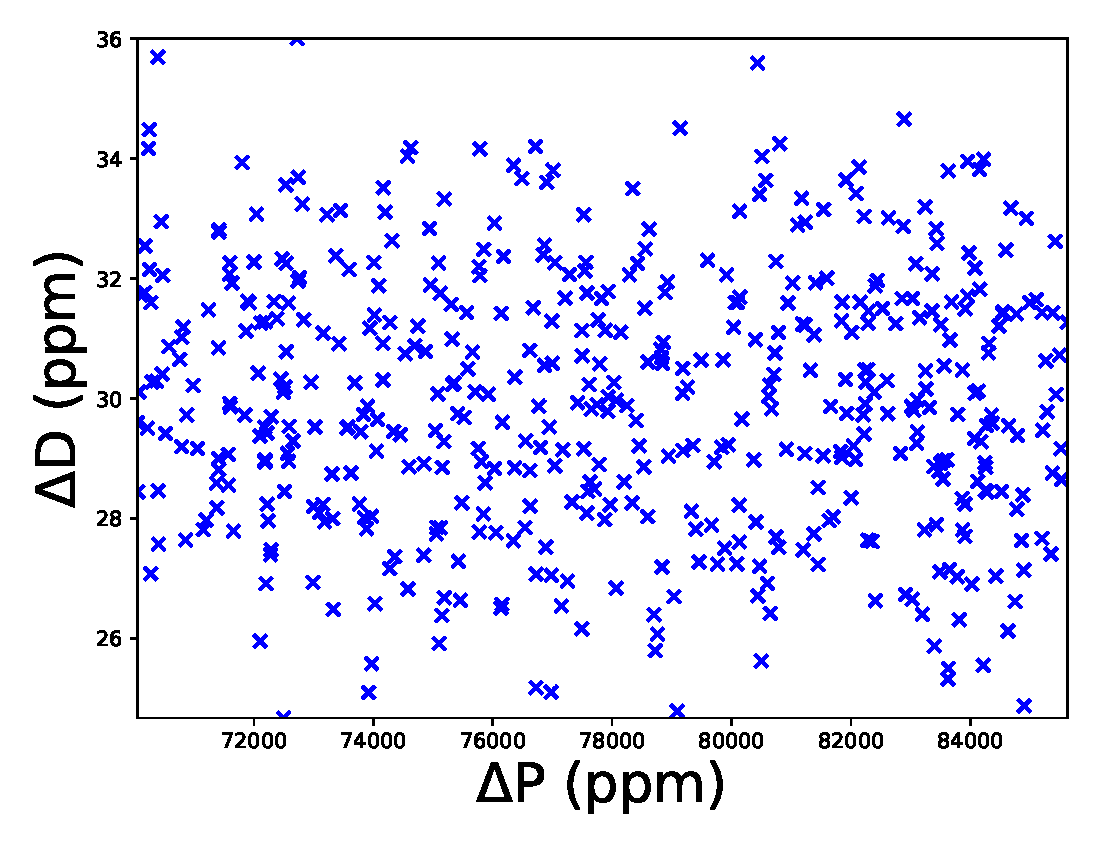
\includegraphics[width=1.0\textwidth]{synthetic_correlation_reflect_vary.eps}
\caption{Examining the correlation between the eclipse depth and transit depth parameters in the presence of variability, these data points represent the uncertainties of the two parameters for each fit performed. The uncertainty in the eclipse depth is plotted on the vertical axis against the uncertainty in the transit depth on the horizontal axis. Synthetic data was generated to mimic the nature of the Quarter-2 Kepler data, where each trial set these two model parameters to randomly vary within plus or minus ten percent of the standard values as obtained in Jackson (2012). For each trial, each set of synthetic data was fit to re-obtain the parameter values and uncertainties. The plot does not appear to reveal any notable correlation between these parameters, where the distribution is evenly spread out.}

\end{figure}

\begin{figure}

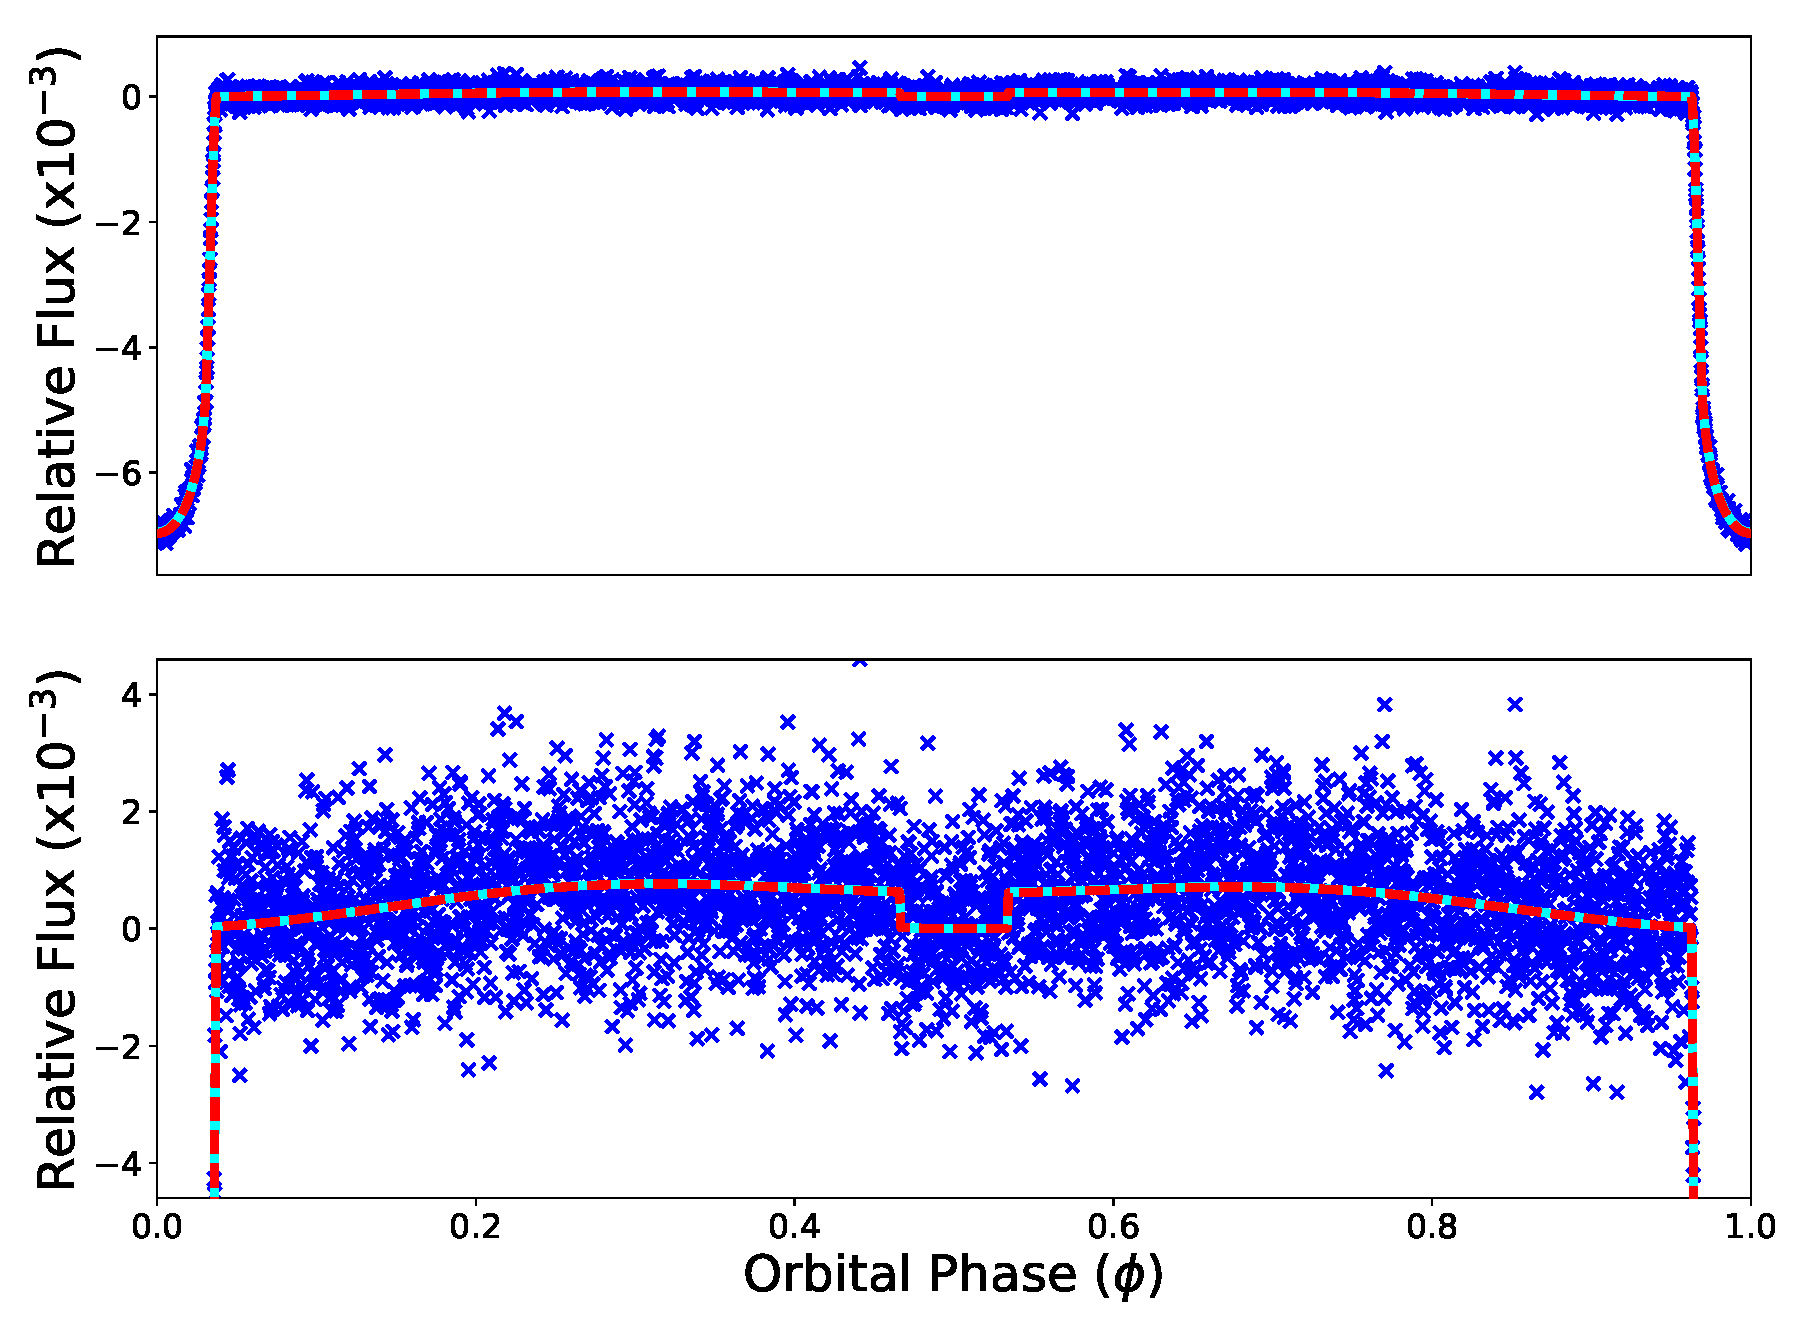
\includegraphics[width=1.0\textwidth]{synthetic_fits_reflect_vary.eps}
\caption{A single result from the synthetic correlation test of the eclipse depth and transit depth parameters. Both plots show the relative flux plotted on the vertical axis versus the orbital phase position on the horizontal axis, where the identical result is shown on different scales to distinguish the transit above and the occultation below. The synthetic data is shown as the blue crosses, the solid cyan line is the model curve with the parameters used, and the dashed red line is the best fit model curve. }

\end{figure}


\begin{figure}

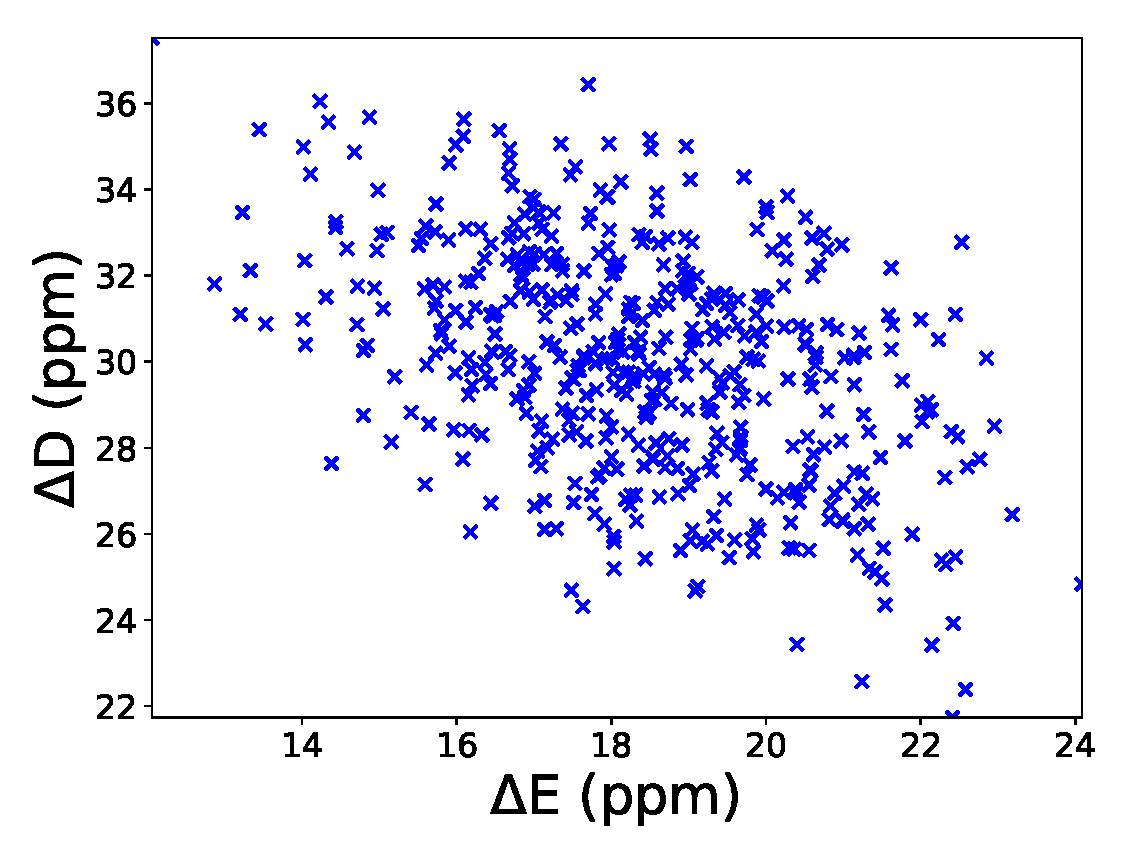
\includegraphics[width=1.0\textwidth]{synthetic_correlation_ellipsoidal_vary.eps}
\caption{Examining the correlation between the eclipse depth and ellipsoidal variation parameters in the presence of variability, these data points represent the uncertainties of the two parameters for each fit performed. The uncertainty in the eclipse depth is plotted on the vertical axis against the uncertainty in the ellipsoidal variation parameter on the horizontal axis. Synthetic data was generated to mimic the nature of the Quarter-2 Kepler data, where each trial set these two model parameters to randomly vary within plus or minus ten percent of the standard values as obtained in Jackson (2012). For each trial, each set of synthetic data was fit to re-obtain the parameter values and uncertainties. The plot appears to show that there is a distinguishable linear trend present, where variability in the eclipse depth appears to be correlated to variability in the ellipsoidal variations.}

\end{figure}

\begin{figure}

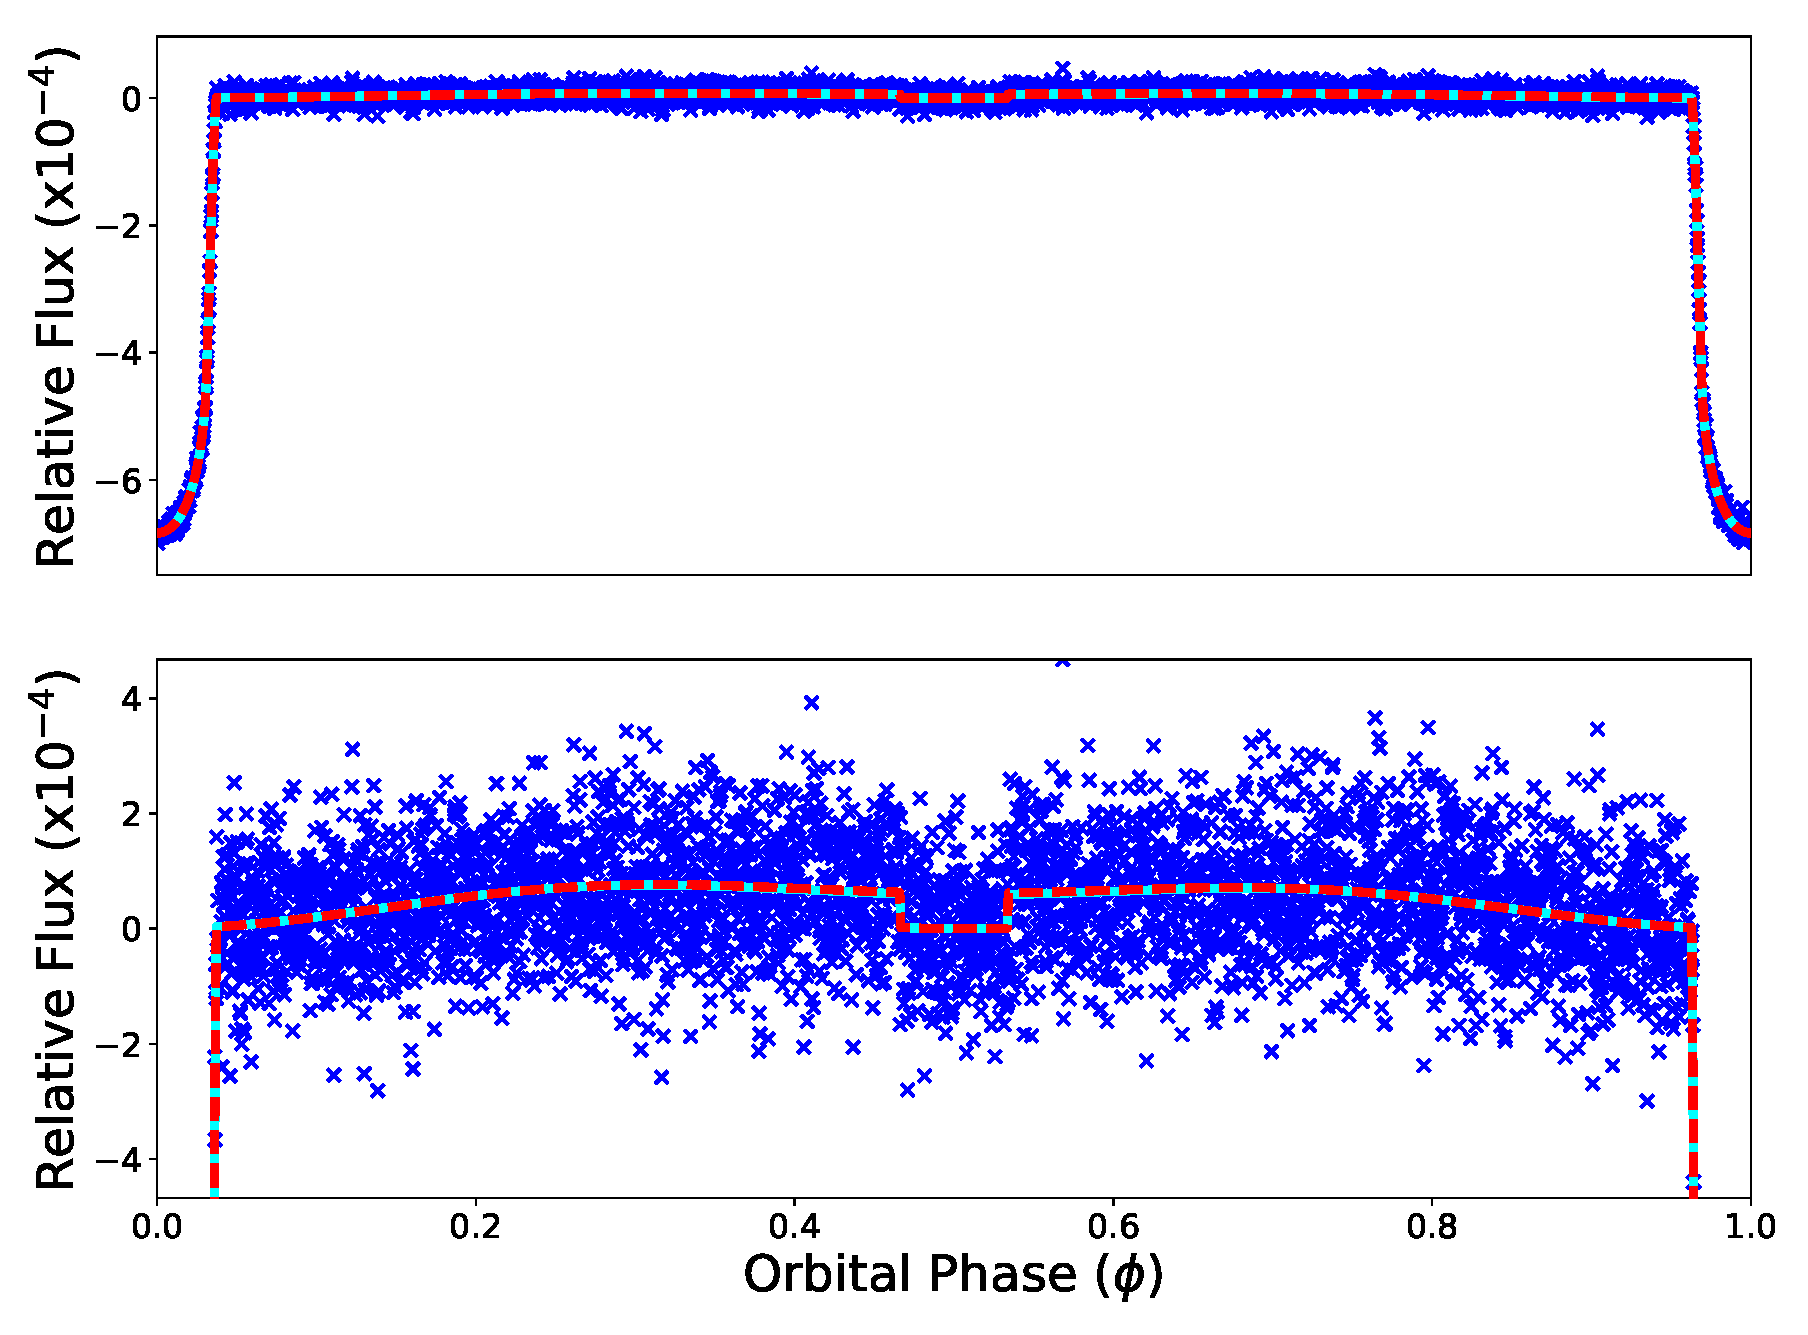
\includegraphics[width=1.0\textwidth]{synthetic_fits_ellipsoidal_vary.eps}
\caption{A single result from the synthetic correlation test of the eclipse depth and ellipsoidal variation parameters. Both plots show the relative flux plotted on the vertical axis versus the orbital phase position on the horizontal axis, where the identical result is shown on different scales to distinguish the transit above and the occultation below. The synthetic data is shown as the blue crosses, the solid cyan line is the model curve with the parameters used, and the dashed red line is the best fit model curve.}

\end{figure}


\begin{figure}

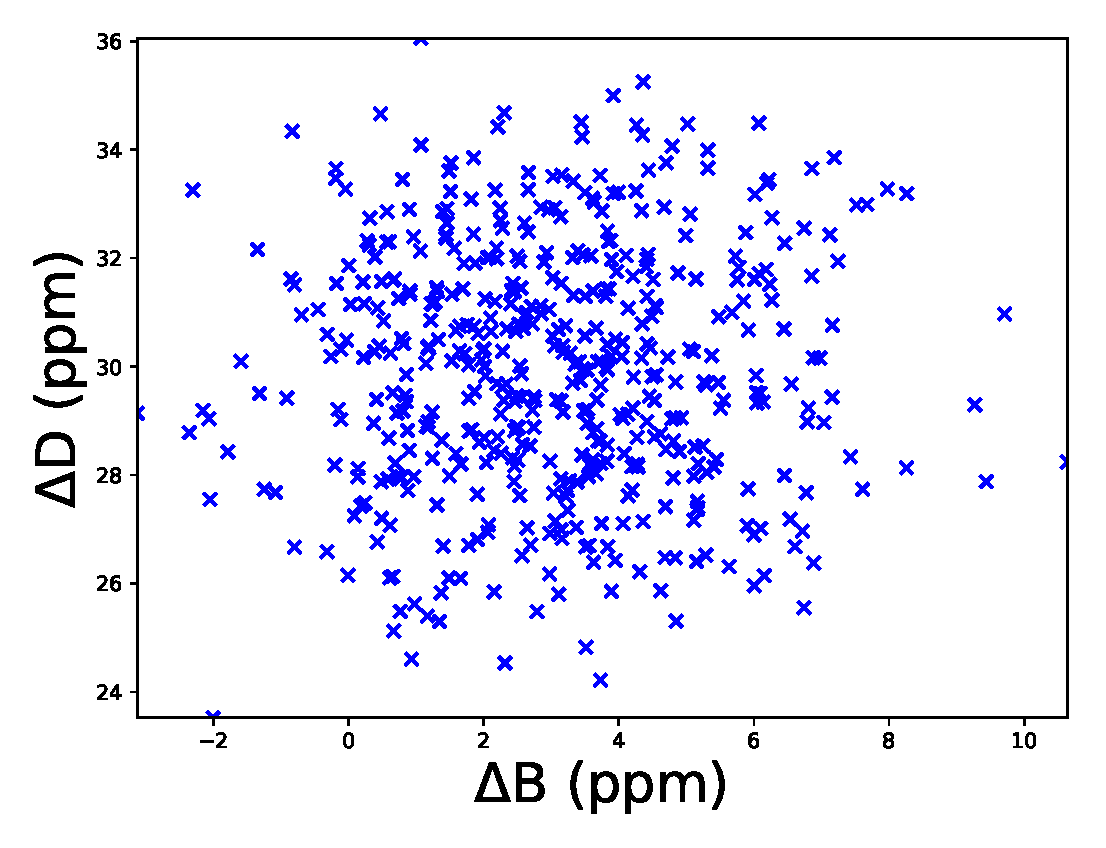
\includegraphics[width=1.0\textwidth]{synthetic_correlation_beaming_vary.eps}
\caption{Examining the correlation between the eclipse depth and Doppler beaming parameters in the presence of variability, these data points represent the uncertainties of the two parameters for each fit performed. The uncertainty in the eclipse depth is plotted on the vertical axis against the uncertainty in the Doppler beaming parameter on the horizontal axis. Synthetic data was generated to mimic the nature of the Quarter-2 Kepler data, where each trial set these two model parameters to randomly vary within plus or minus ten percent of the standard values as obtained in Jackson (2012). For each trial, each set of synthetic data was fit to re-obtain the parameter values and uncertainties. The plot appears to show an even distribution, which suggests that there is no notable correlation between the eclipse and Doppler beaming parameters in the presence of variability.}

\end{figure}

\begin{figure}

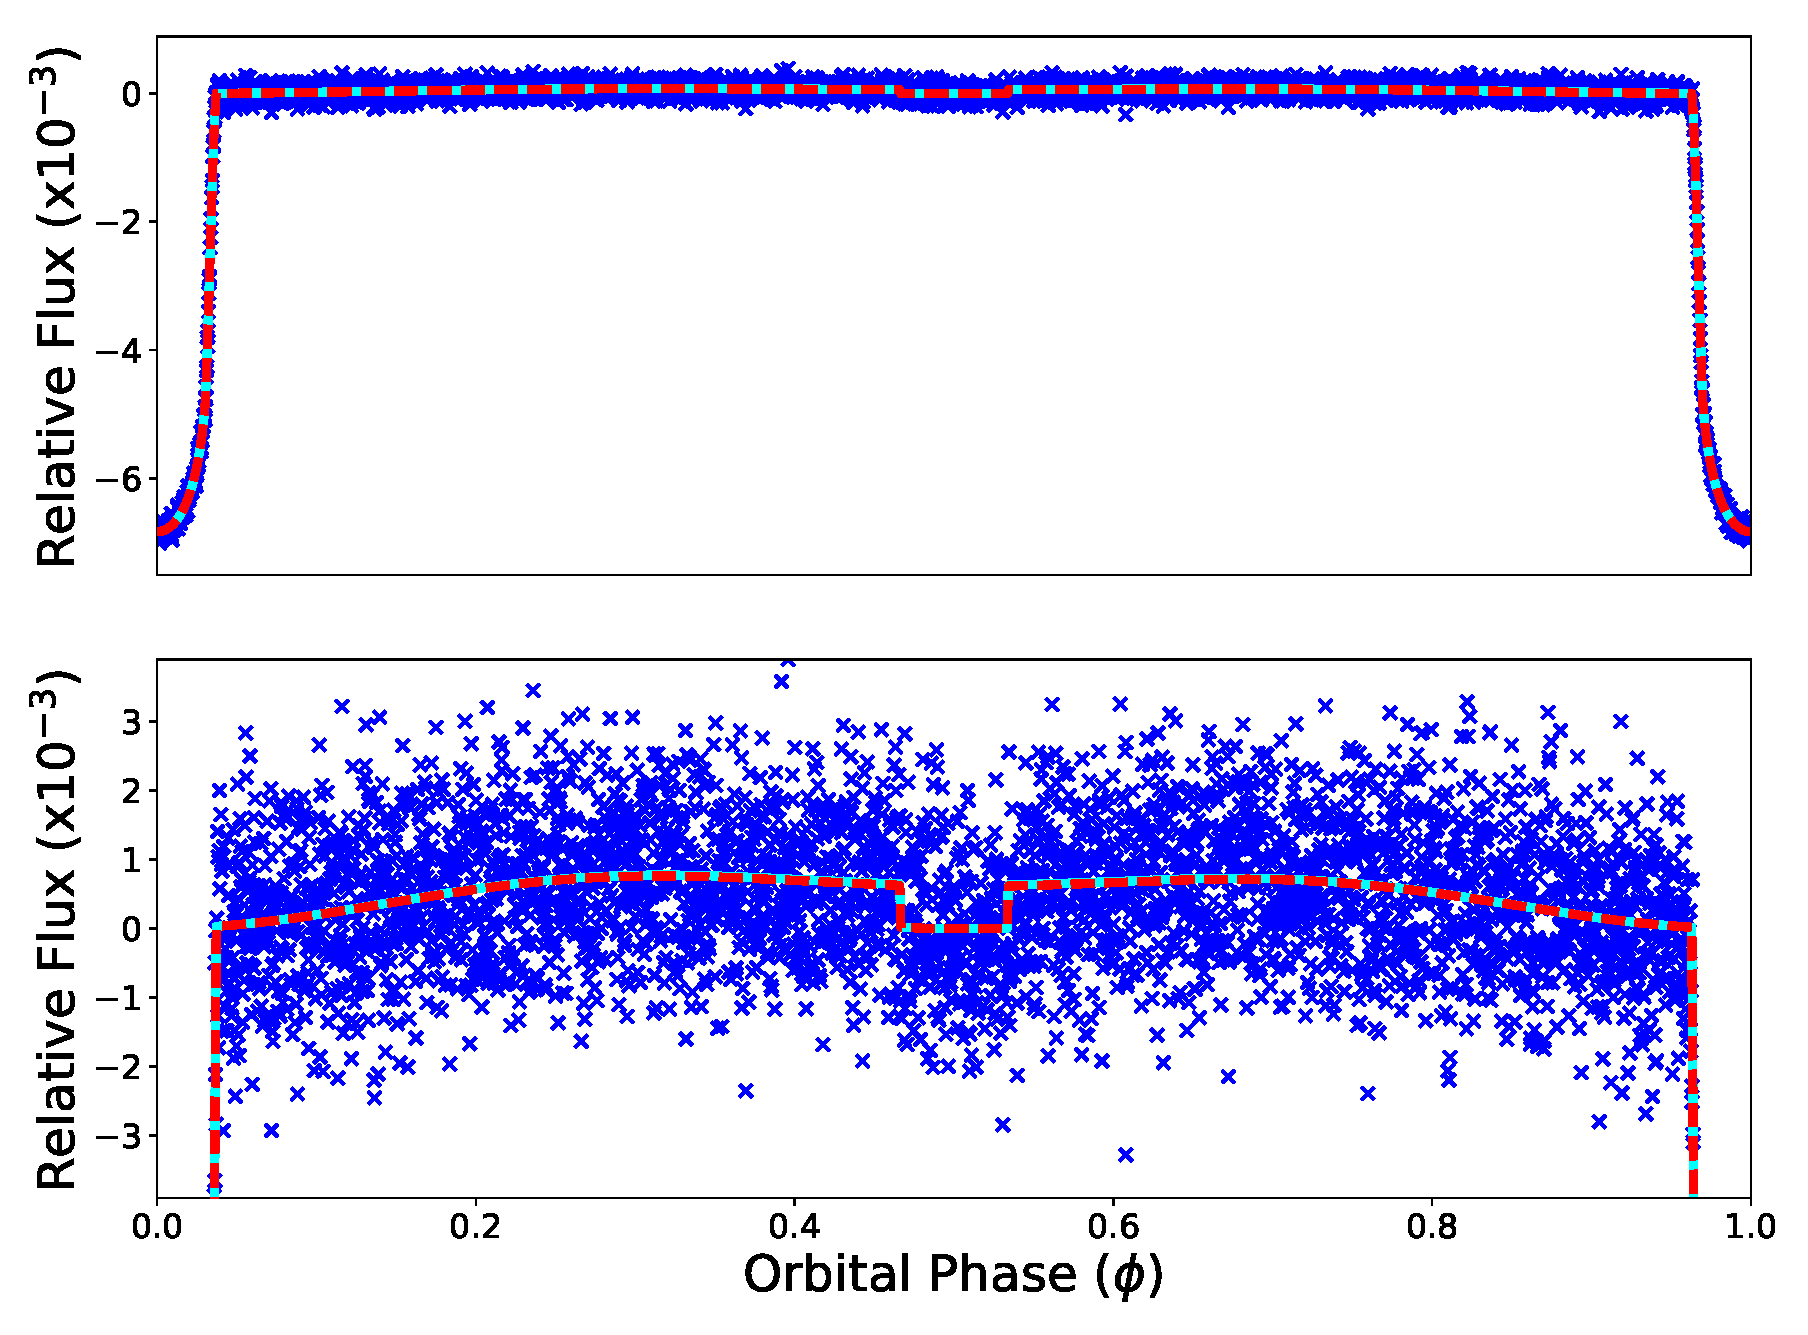
\includegraphics[width=1.0\textwidth]{synthetic_fits_beaming_vary.eps}
\caption{A single result from the synthetic correlation test of the eclipse depth and Doppler beaming parameters. Both plots show the relative flux plotted on the vertical axis versus the orbital phase position on the horizontal axis, where the identical result is shown on different scales to distinguish the transit above and the occultation below. The synthetic data is shown as the blue crosses, the solid cyan line is the model curve with the parameters used, and the dashed red line is the best fit model curve.}

\end{figure}

\begin{figure}

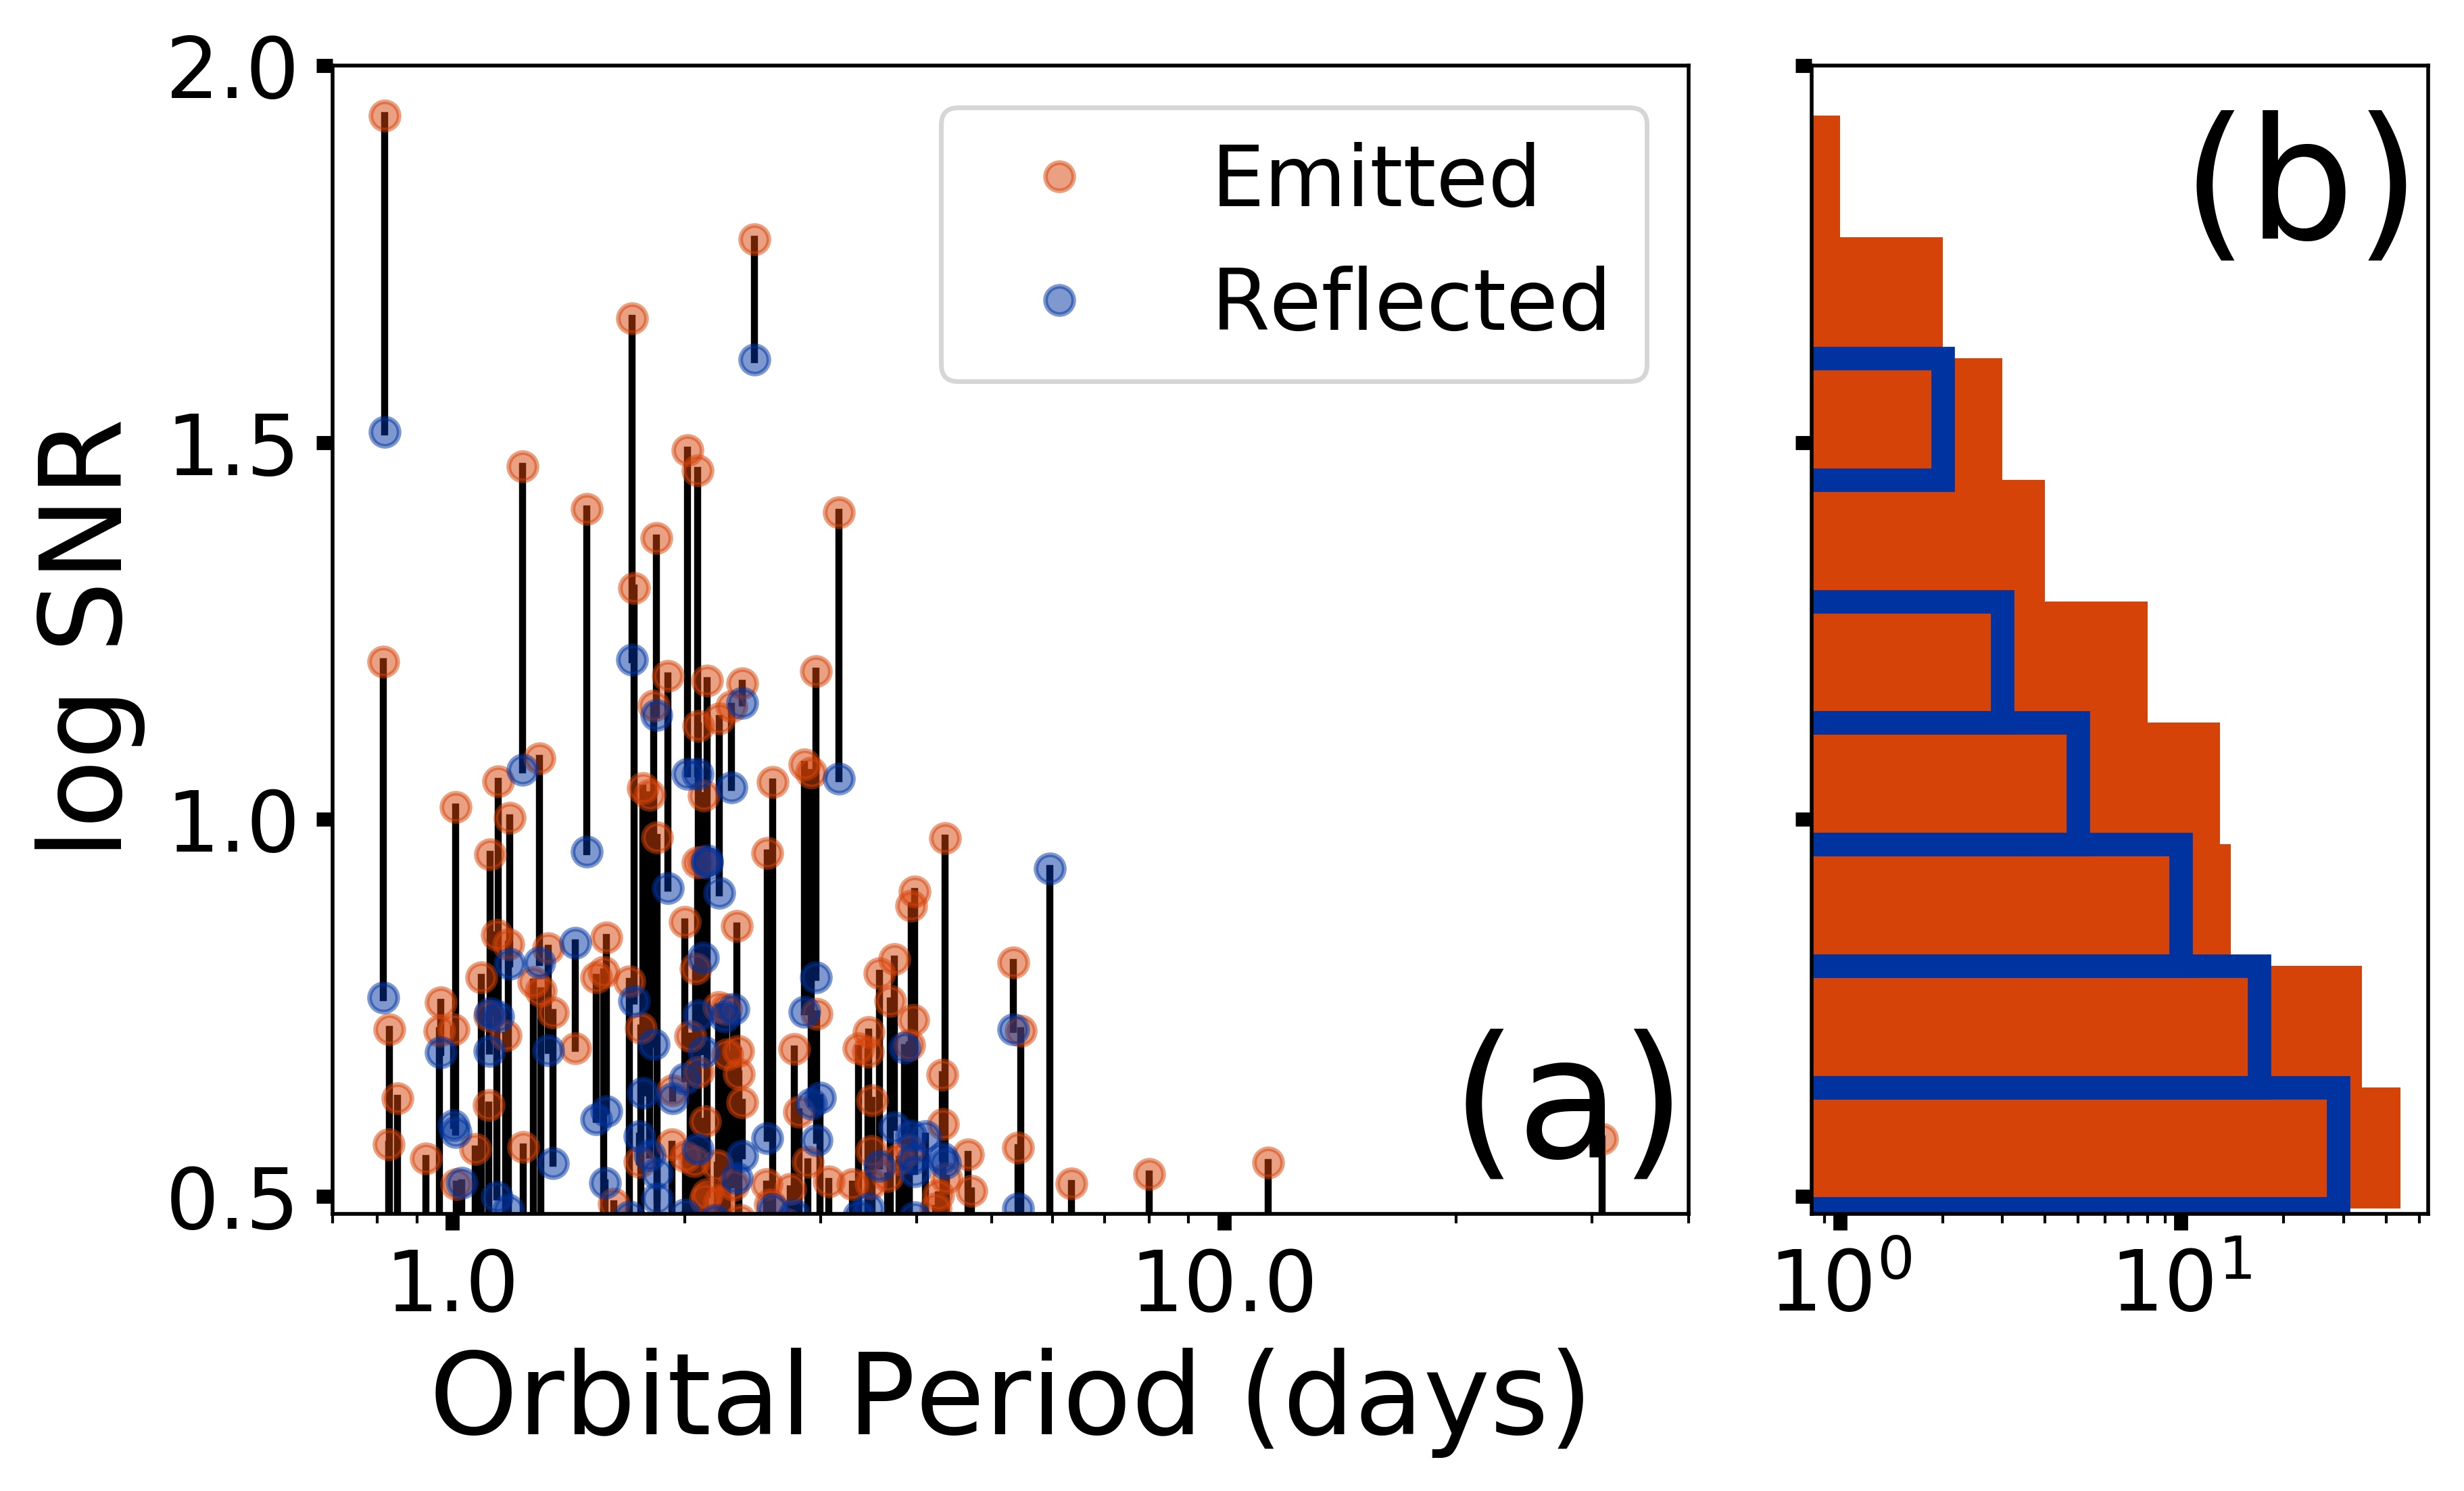
\includegraphics[width=\textwidth]{eclipse_estimates.jpg}
\caption{The $\log$ of the signal-to-noise ratio $SNR$ for planetary secondary eclipses for a population of synthetic planets from the \tess\ mission yield study of \citet{2018arXiv180405050B}. The blue dots in (a)  show eclipses for perfectly reflecting planets, while the orange dots show eclipses for perfect blackbody planets, with black lines connecting the two eclipses for each planet. Panel (b) shows a histogram of SNR-values. \label{fig:eclipse_estimates}}

\end{figure}

\end{document}

%%
%% End of file `sample.tex'.